\section{Task 1: N-Queens -- Propositional Logic and Local Search}

\subsection{Propositional Formulation and CNF Conversion}
We formulate the $N$-Queens problem using $N^2$ Boolean variables $x_{r,c}$ ($0 \le r, c < N$), where $x_{r,c} = \text{True}$ iff a queen is placed at row $r$, column $c$ (encoded with DIMACS identifier $rN + c + 1$).

To systematically discover all placement constraints, we partition the $N\times N$ board into four families of collinear squares: (i)~$N$ rows $R_r = \{x_{r,c} \mid 0 \le c < N\}$, (ii)~$N$ columns $C_c = \{x_{r,c} \mid 0 \le r < N\}$, (iii)~$2N-1$ main diagonals $D^-_d = \{x_{r,c} \mid r - c = d\}$, and (iv)~$2N-1$ anti-diagonals $D^+_s = \{x_{r,c} \mid r + c = s\}$. The constraints are converted directly into Conjunctive Normal Form (CNF) as follows:
\begin{itemize}
  \item \textbf{At-least-one (ALO):} Every row and column must contain at least one queen, yielding $2N$ disjunctions $\bigvee_{c=0}^{N-1} x_{r,c}$ and $\bigvee_{r=0}^{N-1} x_{r,c}$.
  \item \textbf{At-most-one (AMO):} No two distinct squares $a, b$ on the same line $L \in \{R_r, C_c, D^-_d, D^+_s\}$ may both hold a queen. The pairwise exclusion $\neg(a \land b)$ (equivalently $a \rightarrow \neg b$) converts via De Morgan's law into the binary CNF clause $(\neg a \lor \neg b)$ for all $\binom{|L|}{2}$ pairs in $L$.
\end{itemize}
The exact clause count is
$2N + 2N\binom{N}{2} + 2\bigl(2\sum_{k=1}^{N-1}\binom{k}{2}+\binom{N}{2}\bigr) = \Theta(N^3)$.
We pass the CNF clauses to Glucose3 (PySAT), decode positive literals back to $(r, c)$, and verify each solution independently.

\subsection{Min-Conflicts with Age-Biased Variable Selection}
We represent the state as $\text{queens}[c] = r$ (one queen per column), eliminating column conflicts by construction. Incremental row and diagonal counters evaluate the conflicts of any cell $(r,c)$ in $O(1)$. At each iteration, a conflicted column is moved to a minimum-conflict row (with random tie-breaking), restarting after a step budget.
We compare three variable-selection rules: \emph{random} (standard Min-Conflicts), \emph{max-conflict}, and our proposed \emph{oldest} heuristic, which selects a conflicted column maximizing $\text{conflicts} \times (1 + \text{age}/N)$, where $\text{age}$ is the number of steps since that column was last moved. Weighting conflicts by age spreads repairs across the board and mitigates plateau cycling. We also compare random initialization against greedy minimum-conflict initialization.

\subsection{Experiments and Discussion}
We evaluated Glucose3 for $N \in [4, 50]$ and all six Min-Conflicts configurations for $N \in [8, 1000]$ (20 runs per setting). Table~\ref{tab:t1_sat}, Table~\ref{tab:t1_mc}, Fig.~\ref{fig:t1_sat}, and Fig.~\ref{fig:t1_mc} summarize the results.

\begin{table}[htbp]
\centering
\caption{Glucose3 SAT Performance on $N$-Queens (seconds).}
\label{tab:t1_sat}
\begin{tabular}{rrrrr}
\hline
$N$ & \#Vars & \#Clauses & Encode (s) & Solve (s) \\
\hline
4  & 16       & 84        & 0.0001 & 0.0016 \\
8  & 64       & 744       & 0.0003 & 0.0010 \\
16 & 256      & 6{,}352   & 0.0064 & 0.0199 \\
24 & 576      & 21{,}944  & 0.0051 & 0.0800 \\
32 & 1{,}024  & 52{,}640  & 0.0140 & 0.0351 \\
40 & 1{,}600  & 103{,}560 & 0.0550 & 0.0654 \\
50 & 2{,}500  & 203{,}450 & 0.0855 & 0.1154 \\
\hline
\end{tabular}
\end{table}

\begin{table}[htbp]
\centering
\caption{Min-Conflicts Performance at $N=1000$ (20 runs, 100\% success).}
\label{tab:t1_mc}
\begin{tabular}{llrrr}
\hline
Variable & Init & Mean Steps & Median & Time (s) \\
\hline
random       & random & 710.2 & 709.0 & 0.3689 \\
max-conflict & random & 563.1 & 558.0 & 0.3704 \\
oldest       & random & 537.7 & 539.5 & 0.3600 \\
random       & greedy &  82.3 &  85.5 & 0.2656 \\
max-conflict & greedy &  81.6 &  83.0 & 0.2633 \\
oldest       & greedy &  49.1 &  44.0 & 0.2363 \\
\hline
\end{tabular}
\end{table}

\begin{figure}[htbp]
\centerline{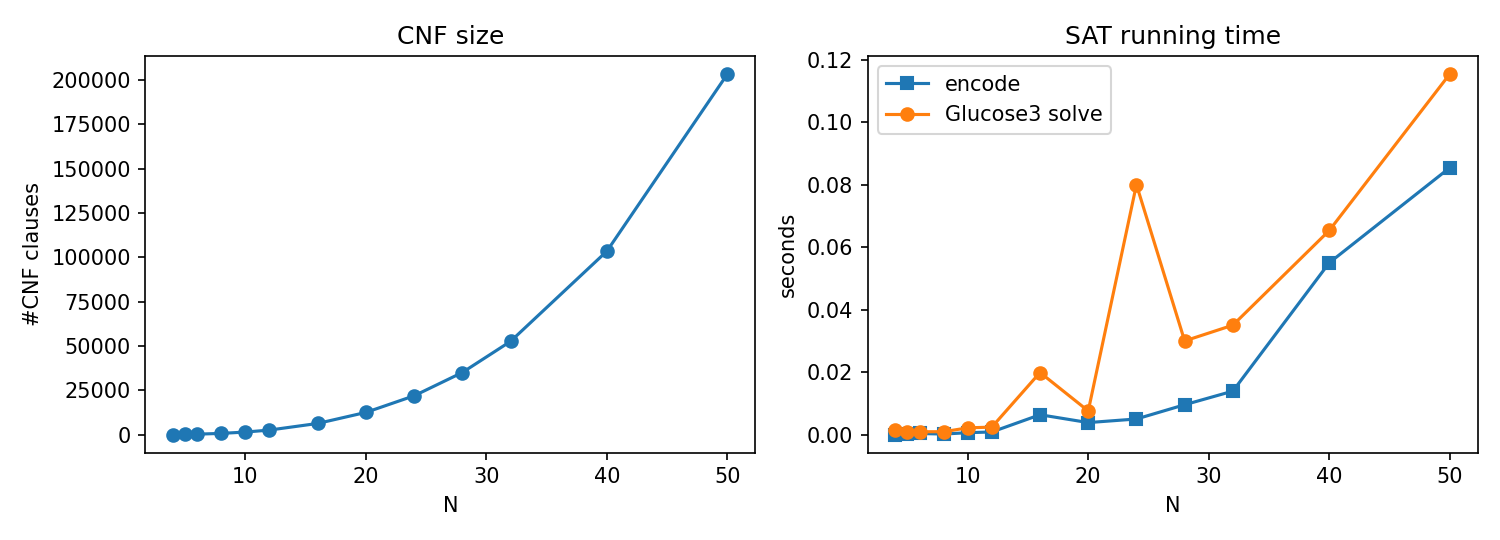
\includegraphics[width=\columnwidth]{results/sat_scaling.png}}
\caption{CNF clause growth and Glucose3 encoding/solving time vs.\ $N$.}
\label{fig:t1_sat}
\end{figure}

\begin{figure}[htbp]
\centerline{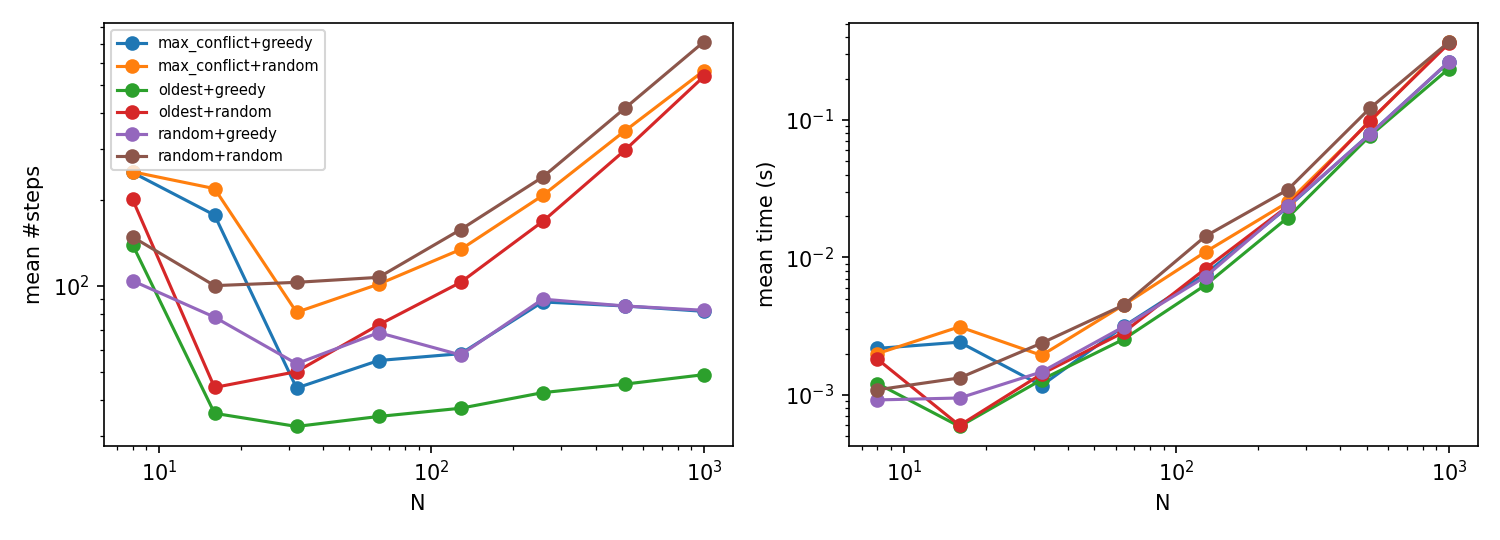
\includegraphics[width=\columnwidth]{results/mc_heuristics.png}}
\caption{Min-Conflicts mean steps and runtime across heuristics and initializations (log-log scale, 20 runs).}
\label{fig:t1_mc}
\end{figure}

Although the pairwise CNF encoding grows cubically to $203{,}450$ clauses at $N=50$, Glucose3 solves every tested instance validly in at most $0.2009\text{ s}$ total time (with mild non-monotonicity in CDCL search time, e.g., $N=24$ vs.\ $N=32$). For large $N$, Min-Conflicts achieves a $100\%$ success rate across all runs and scales smoothly to $N=1000$ in under $0.4\text{ s}$. At $N=1000$, greedy initialization alone reduces standard \emph{random} Min-Conflicts steps by $88.4\%$ ($710.2$ to $82.3$), while our proposed \emph{oldest} heuristic further lowers the step count to $49.1$ ($40.3\%$ fewer steps than \emph{random+greedy} and $93.1\%$ fewer than standard \emph{random+random}), cutting mean runtime by $35.9\%$ ($0.3689\text{ s}$ to $0.2363\text{ s}$). Across all board sizes $N \ge 16$, \emph{oldest+greedy} consistently requires the fewest repair steps.